\documentclass[11pt,a4paper]{article}

% ── Packages ──────────────────────────────────────────────────────────────
\usepackage[utf8]{inputenc}
\usepackage[T1]{fontenc}
\usepackage{lmodern}
\usepackage[margin=2.4cm]{geometry}
\usepackage{amsmath,amssymb,amsthm}
\usepackage{mathtools}
\usepackage{booktabs}
\usepackage{enumitem}
\usepackage{algorithm}
\usepackage{algpseudocode}
\usepackage{hyperref}
\usepackage{xcolor}
\usepackage{graphicx}
\usepackage{caption}
\usepackage{subcaption}
\usepackage{tikz}
\usetikzlibrary{arrows.meta,positioning,calc}

\hypersetup{
    colorlinks=true,
    linkcolor=blue!60!black,
    citecolor=blue!60!black,
    urlcolor=blue!60!black,
}

% ── Theorem environments ──────────────────────────────────────────────────
\newtheorem{definition}{Definition}
\newtheorem{remark}{Remark}

% ── Macros ────────────────────────────────────────────────────────────────
\newcommand{\R}{\mathbb{R}}
\newcommand{\E}{\mathbb{E}}
\newcommand{\Var}{\mathrm{Var}}
\newcommand{\Ind}{\mathbf{1}}
\newcommand{\cF}{\mathcal{F}}
\DeclareMathOperator*{\argmax}{arg\,max}

% ── Colors for agent types ────────────────────────────────────────────────
\definecolor{cEarly}{HTML}{2196F3}
\definecolor{cInformed}{HTML}{4CAF50}
\definecolor{cMomentum}{HTML}{FF9800}
\definecolor{cOption}{HTML}{9C27B0}
\definecolor{cNoise}{HTML}{9E9E9E}
\definecolor{cWhale}{HTML}{F44336}

% ══════════════════════════════════════════════════════════════════════════
\title{\textbf{Continuous Clearing Auction Simulator}\\[4pt]
       \large Agent-Based Model: Architecture and Mechanics}
\author{Kosmos Ventures}
\date{\today}

\begin{document}
\maketitle

% ──────────────────────────────────────────────────────────────────────────
\begin{abstract}
We describe the design and implementation of an agent-based simulation of the Continuous Clearing Auction (CCA), a time-discretized uniform-price mechanism for onchain token sales.
The simulator faithfully implements the mathematical model of the CCA—including deterministic supply schedules, proportional budget spreading, and uniform-price clearing via bisection—and populates it with six heterogeneous agent types whose behavioural rules encode the key economic forces identified in the theoretical analysis: the \emph{exposure premium} of early entry (Proposition~1) versus the \emph{informational option value} of delay (Proposition~2).
A Monte Carlo and parameter-sweep infrastructure enables systematic exploration of how sentiment, demand intensity, information leakage, supply shape, and agent composition jointly determine clearing prices, surplus allocation, and participation dynamics.
\end{abstract}

\tableofcontents
\newpage

% ══════════════════════════════════════════════════════════════════════════
\section{Introduction and Motivation}
\label{sec:intro}

A \emph{Continuous Clearing Auction} (CCA) generalises the familiar single-shot uniform-price auction to a setting in which supply is released over a sequence of discrete periods and the market clears repeatedly. The mechanism is designed for onchain token sales and aims to eliminate the incentive to delay participation that plagues standard uniform-price formats.

The theoretical analysis establishes two competing forces:
\begin{enumerate}[label=(\roman*)]
  \item \textbf{Exposure premium.}  Entering earlier expands the support of a bidder's budget schedule across more clearing periods, granting access to potentially high-surplus early clearings.  When per-dollar surplus is front-loaded (weakly decreasing in time), early entry weakly dominates (Proposition~1).
  \item \textbf{Informational option value.}  When external information leakage refines beliefs about the fundamental value~$V$ or the future clearing-price path, delaying entry allows conditioning on improved signals.  If the conditional surplus can change sign, optimal stopping with delayed entry strictly dominates unconditional commitment (Proposition~2).
\end{enumerate}

The simulator instantiates both regimes through a heterogeneous population of agents and measures how the balance between these forces varies with market parameters.

This document describes:
\begin{itemize}[nosep]
  \item the CCA mechanism as implemented (Section~\ref{sec:mechanism});
  \item the agent taxonomy and behavioural rules (Section~\ref{sec:agents});
  \item the information and sentiment environment (Section~\ref{sec:information});
  \item the simulation loop and Monte Carlo infrastructure (Section~\ref{sec:orchestration});
  \item the experimental design and parameter sweeps (Section~\ref{sec:experiments}).
\end{itemize}


% ══════════════════════════════════════════════════════════════════════════
\section{CCA Mechanism}
\label{sec:mechanism}

% ─────────────────────────────────────────────────────────
\subsection{Time and Supply}
\label{sec:supply}

Time is discrete, indexed by~$k \in \{1,\dots,T\}$.  The auctioneer commits \emph{ex ante} to a deterministic supply-release schedule: at each period~$k$ a token increment~$q_k > 0$ is released, with total supply
\[
  Q \;=\; \sum_{k=1}^{T} q_k.
\]

The schedule is constructed from a weight vector~$\mathbf{w} = (w_1,\dots,w_T)$ via normalisation:
\begin{equation}\label{eq:supply-normalise}
  q_k \;=\; Q \cdot \frac{w_k}{\sum_{j=1}^{T} w_j}.
\end{equation}

Five parametric families are supported:

\begin{table}[h]
\centering
\caption{Supply schedule types.}
\label{tab:supply}
\begin{tabular}{@{}lll@{}}
\toprule
\textbf{Type} & \textbf{Weight formula} & \textbf{Intuition} \\
\midrule
\texttt{uniform}       & $w_k = 1$                                              & Constant release \\
\texttt{front\_loaded} & $w_k = \operatorname{linspace}(2.0,\,0.2,\,T)_k$      & Heavy early release \\
\texttt{back\_loaded}  & $w_k = \operatorname{linspace}(0.2,\,2.0,\,T)_k$      & Heavy late release \\
\texttt{bell\_curve}   & $w_k = \exp\!\bigl(-\tfrac{1}{2}x_k^2\bigr)$,\; $x \in [-3,3]$ & Peak in middle \\
\texttt{custom}        & User-provided vector                                    & Arbitrary \\
\bottomrule
\end{tabular}
\end{table}


% ─────────────────────────────────────────────────────────
\subsection{Bids and Spreading Rule}
\label{sec:spreading}

A bidder submits a budget~$B > 0$ (in the quote asset) and a maximum acceptable unit price (cap)~$m \in (0,\infty]$ at an entry time~$\tau$.  The mechanism maps this bid into a \emph{budget schedule}~$\bigl(b_k(\tau)\bigr)_{k=1}^{T}$ satisfying:
\begin{equation}\label{eq:spreading-constraints}
  b_k(\tau) \geq 0, \qquad
  \sum_{k=\tau}^{T} b_k(\tau) = B, \qquad
  b_k(\tau) = 0 \;\;\text{for } k < \tau.
\end{equation}

The default (canonical) spreading rule is \textbf{proportional-to-remaining-supply}:
\begin{equation}\label{eq:proportional-spread}
  b_k(\tau) \;=\; B \cdot \frac{q_k}{\displaystyle\sum_{j=\tau}^{T} q_j}, \qquad k \geq \tau.
\end{equation}

This allocates budget to each future period in proportion to that period's share of the remaining supply.  Two alternative rules are also implemented for sensitivity analysis:
\begin{itemize}[nosep]
  \item \textbf{Equal-weight}: $b_k(\tau) = B/(T - \tau)$ for $k \geq \tau$.
  \item \textbf{Front-weighted} (geometric decay $\delta$): $b_k(\tau) \propto \delta^{k-\tau}$, normalised to sum to~$B$.
\end{itemize}

The spreading rule interface is pluggable: any function mapping a bid and supply schedule to a conforming budget vector can be substituted.


% ─────────────────────────────────────────────────────────
\subsection{Uniform-Price Clearing}
\label{sec:clearing}

At each period~$k$, the mechanism performs the following steps:

\begin{enumerate}[nosep]
  \item \textbf{Collect active fragments.}  For every bid~$i$ with entry time $\tau_i \leq k$, the budget fragment is~$b_k^{(i)} = b_k(\tau_i)$.
  \item \textbf{Aggregate demand curve.}  At candidate price~$p$, bid~$i$ demands
  \[
    d_k^{(i)}(p) \;=\; \frac{b_k^{(i)}}{p}\,\Ind\{p \leq m_i\}
  \]
  tokens.  Total demand is
  \begin{equation}\label{eq:demand}
    D_k(p) \;=\; \sum_{i} d_k^{(i)}(p) \;=\; \frac{1}{p}\sum_{i:\,m_i \geq p} b_k^{(i)}.
  \end{equation}
  Note that $D_k(\cdot)$ is monotone decreasing in~$p$ within each piece between consecutive caps.

  \item \textbf{Find the clearing price.}  The uniform clearing price~$P_k$ solves $D_k(P_k) = q_k$.  Since~$D_k$ is monotone decreasing, this is found by \textbf{bisection} on the interval $[p_{\min}, p_{\max}]$ with tolerance $10^{-8}$ and a maximum of 200 iterations.

  \item \textbf{Execute.}  Each bid~$i$ with $P_k \leq m_i$ spends~$b_k^{(i)}$ and receives $b_k^{(i)} / P_k$ tokens.  Bids with $P_k > m_i$ do not transact; their fragment goes unspent.
\end{enumerate}

\paragraph{Edge cases.}
\begin{itemize}[nosep]
  \item If $D_k(p_{\min}) \leq q_k$ (total demand below supply even at the floor), set $P_k = p_{\min}$.
  \item If $D_k(p_{\max}) \geq q_k$ (excess demand at the ceiling), set $P_k = p_{\max}$.
  \item If no bids are active, $P_k$ defaults to~$p_{\min}$.
\end{itemize}


% ─────────────────────────────────────────────────────────
\subsection{Surplus Computation}
\label{sec:surplus}

For each bid~$i$ with valuation~$V^{(i)}$, the per-period realised surplus at period~$k$ is:
\begin{equation}\label{eq:surplus-period}
  \pi_k^{(i)}(\tau, m) \;=\; \Ind\{P_k \leq m\}\left(\frac{V^{(i)}}{P_k} - 1\right) b_k(\tau).
\end{equation}

The term $V^{(i)}/P_k - 1$ is the surplus per dollar spent: spending $b_k$ at price~$P_k$ buys $b_k / P_k$ tokens, each worth~$V^{(i)}$, yielding a dollar profit of $(V^{(i)} - P_k) \cdot b_k / P_k = (V^{(i)}/P_k - 1)\,b_k$.

Total surplus aggregates across all periods of participation:
\begin{equation}\label{eq:surplus-total}
  \Pi^{(i)} \;=\; \sum_{k=\tau}^{T} \pi_k^{(i)}(\tau, m).
\end{equation}

For each bid, the simulator records: per-period surplus array, total surplus, total tokens acquired, total spend, unspent budget, budget-weighted average execution price, and surplus per dollar spent.


% ══════════════════════════════════════════════════════════
\section{Agent Taxonomy}
\label{sec:agents}

The simulation populates the CCA with six agent types, each encoding a distinct behavioural regime.  All agents share a common state and belief-update mechanism, but differ in entry logic, cap selection, and—in some cases—belief-formation overrides.

% ─────────────────────────────────────────────────────────
\subsection{Common Agent State}
\label{sec:agent-state}

Every agent~$i$ maintains:
\begin{itemize}[nosep]
  \item Budget $B^{(i)} > 0$ in the quote asset.
  \item Base valuation $V^{(i)}_{\text{base}}$ (prior fundamental value) and uncertainty $\sigma_V$.
  \item Running posterior: belief mean $\hat{\mu}$ and variance $\hat{\sigma}^2$.
  \item Current valuation $\hat{V}^{(i)} = \hat{\mu}$ (set after each belief update).
  \item Sentiment sensitivity~$\gamma_i \in (0,\infty)$, controlling weight on public signals.
  \item Entry state: whether the agent has entered, and if so, the entry period~$\tau_i$.
\end{itemize}

% ─────────────────────────────────────────────────────────
\subsection{Market State Observable}
\label{sec:market-state}

At each period~$k$, every agent observes a \texttt{MarketState} object containing: the current period; the history of clearing prices $P_0,\dots,P_{k-1}$; cumulative and remaining supply; the full supply schedule~$(q_k)$; the current public signal~$s_k$; the aggregate sentiment index~$\sigma_k \in [0,1]$; and the realised log-price volatility.

% ─────────────────────────────────────────────────────────
\subsection{Default Belief Update}
\label{sec:belief-update}

Unless overridden by a specific agent type, every agent performs a \emph{two-stage conjugate-normal update} each period.

\paragraph{Stage~1: Public signal update.}
Define the prior precision $\lambda_{\text{prior}} = 1/\hat{\sigma}^2$ and the signal precision $\lambda_{\text{sig}} = \gamma / \sigma_V^2$, where $\gamma$ is the agent's sentiment sensitivity.  Given public signal~$s_k$:
\begin{equation}\label{eq:belief-stage1}
  \hat{\mu}_{\text{post}} = \frac{\lambda_{\text{prior}}\,\hat{\mu} + \lambda_{\text{sig}}\,s_k}{\lambda_{\text{prior}} + \lambda_{\text{sig}}},
  \qquad
  \hat{\sigma}^2_{\text{post}} = \frac{1}{\lambda_{\text{prior}} + \lambda_{\text{sig}}}.
\end{equation}

\paragraph{Stage~2: Price signal update.}
If a clearing price $P_{k-1} > 0$ is available, it is treated as an additional signal about~$V$ after scaling by a factor of~$1.2\times$ (reflecting that the clearing price is an upward-biased estimator of fundamental value in high-demand settings).  The signal precision is $\lambda_{\text{price}} = 0.5/\nu^2$, where $\nu$ is the realised log-price volatility.  A second conjugate update is applied:
\begin{equation}\label{eq:belief-stage2}
  \hat{\mu}' = \frac{\lambda'_{\text{prior}}\,\hat{\mu}_{\text{post}} + \lambda_{\text{price}} \cdot 1.2 P_{k-1}}{\lambda'_{\text{prior}} + \lambda_{\text{price}}},
  \qquad
  (\hat{\sigma}')^2 = \frac{1}{\lambda'_{\text{prior}} + \lambda_{\text{price}}},
\end{equation}
where $\lambda'_{\text{prior}} = 1/\hat{\sigma}^2_{\text{post}}$.  After updating, the agent sets $\hat{V}^{(i)} = \hat{\mu}'$.


% ─────────────────────────────────────────────────────────
\subsection{Agent Type Specifications}
\label{sec:agent-types}

Each agent type implements three methods: \texttt{decide\_entry}$(k, \text{state}) \to \text{bool}$, \texttt{decide\_cap}$(k, \text{state}) \to \R_{>0}$, and optionally overrides \texttt{update\_beliefs}.

\subsubsection{EarlyBeliever}
\label{sec:early-believer}

\textbf{Concept.}  High-conviction agent that enters very early, corresponding to the regime where Proposition~1 dominates (front-loaded surplus expectation).

\textbf{Parameters} (sampled per agent):
\begin{itemize}[nosep]
  \item $\texttt{conviction\_multiplier} \sim U(1.3,\,1.8)$: scales valuation to set cap.
  \item $\texttt{max\_entry\_delay} \sim \{0,1,2\}$: latest period to enter.
\end{itemize}

\textbf{Entry logic.}  At each period $k \leq \texttt{max\_entry\_delay}$, enter with probability $1 - (0.3 - 0.2\cdot\sigma_k)$, where $\sigma_k$ is the sentiment index.  Entry is forced at the maximum delay period.

\textbf{Cap.}  $m = \hat{V}\cdot\texttt{conviction\_multiplier}$.

\textbf{Beliefs.}  Default (Section~\ref{sec:belief-update}).


\subsubsection{InformedTrader}
\label{sec:informed-trader}

\textbf{Concept.}  Receives private signals about~$V$ and conditions entry on signal quality.  Models the option-value regime of Proposition~2.

\textbf{Parameters:}
\begin{itemize}[nosep]
  \item $\texttt{signal\_precision} \sim U(1,4)$: precision of private signal.
  \item $\texttt{entry\_threshold} \sim U(0.05,0.20)$: minimum expected surplus per dollar.
  \item $\texttt{signal\_delay} \sim \{1,2,3,4\}$: periods before private signal arrives.
\end{itemize}

\textbf{Private signal model.}  At each period $k \geq \texttt{signal\_delay}$, the agent draws
\[
  s^{\text{priv}}_k = V_{\text{base}} + \varepsilon, \qquad \varepsilon \sim \mathcal{N}\!\left(0,\;\frac{1}{\texttt{signal\_precision}}\right),
\]
and performs a Bayesian conjugate update incorporating this private signal on top of the standard two-stage update.

\textbf{Entry logic.}  Wait until $k \geq \texttt{signal\_delay}$.  Estimate expected surplus per dollar as $\hat{\mu}/\hat{P} - 1$, where $\hat{P}$ is the last observed clearing price (or $0.8\,V_{\text{base}}$ as a prior).  Enter if this exceeds a time-decaying threshold:
\[
  \frac{\hat{\mu}}{\hat{P}} - 1 \;>\; \texttt{entry\_threshold} \cdot \frac{T - k}{T}.
\]

\textbf{Cap.}  $m = \hat{V} \cdot 1.1$ (tight cap).


\subsubsection{MomentumTrader}
\label{sec:momentum-trader}

\textbf{Concept.}  FOMO-driven agent that enters on price trend confirmation.

\textbf{Parameters:}
\begin{itemize}[nosep]
  \item $\texttt{lookback} \sim \{2,3,4,5\}$: window for momentum computation.
  \item $\texttt{momentum\_threshold} \sim U(0.01,0.05)$: minimum mean log-return.
  \item $\texttt{fomo\_factor} \sim U(0.5,2.0)$: scales entry probability.
\end{itemize}

\textbf{Momentum.}  Computed as the mean of $\Delta\log P$ over the last \texttt{lookback} valid prices.

\textbf{Entry logic.}
\begin{itemize}[nosep]
  \item If $\textit{momentum} > \texttt{threshold}$, enter with probability $\min\!\bigl(1,\;\texttt{fomo\_factor}\cdot\textit{momentum}/\texttt{threshold}\bigr)$.
  \item \emph{Late-stage panic}: if $k > 0.8\,T$, enter with probability proportional to urgency $= (k - 0.8T)/(0.2T)$, capped at~$0.5$.
\end{itemize}

\textbf{Cap.}  $m = \max(\text{recent\_price}\times 1.2,\;\hat{V})$.

\textbf{Belief override.}  Strong price anchoring: $\hat{V} \leftarrow 0.6\,\hat{V} + 0.4\,P_{k-1}\cdot 1.1$.


\subsubsection{OptionValueOptimizer}
\label{sec:option-value}

\textbf{Concept.}  Explicitly models the exposure premium vs.\ option value tradeoff formalised in Proposition~2.

\textbf{Parameters:}
\begin{itemize}[nosep]
  \item $\texttt{patience} \sim U(0.3,1.0)$: weight on the option-value term.
  \item $\texttt{option\_value\_decay} \sim U(0.75,0.95)$: per-period decay.
\end{itemize}

\textbf{Option value estimate.}  The option value captures the Proposition~2 intuition that the value of waiting is proportional to uncertainty times the square root of remaining time:
\begin{equation}\label{eq:option-value}
  \mathrm{OV}(k) \;=\; \texttt{patience}\;\cdot\;\sqrt{\hat{\sigma}^2}\;\cdot\;\sqrt{T - k}\;\cdot\;\texttt{decay}^{\,k}.
\end{equation}

\textbf{Exposure premium estimate:}
\begin{equation}\label{eq:exposure-premium}
  \mathrm{EP}(k) \;=\; \max\!\left(\frac{\hat{\mu}}{\hat{P}} - 1,\;0\right)\;\cdot\;\frac{q_k}{\sum_{j \geq k} q_j}\;\cdot\; B.
\end{equation}

\textbf{Entry logic.}  Enter when $\mathrm{EP}(k) > \mathrm{OV}(k)$.  If fewer than 15\% of periods remain, enter whenever expected surplus is positive.

\textbf{Cap.}  $m = \hat{V} \cdot 1.05$ (very tight—sophisticated agent).


\subsubsection{NoiseTrader}
\label{sec:noise-trader}

\textbf{Concept.}  Behavioural retail participation: random entry, noisy cap, provides liquidity.

\textbf{Parameters:}
\begin{itemize}[nosep]
  \item $\texttt{entry\_probability} \sim U(0.08,0.28)$: per-period base entry rate.
  \item $\texttt{cap\_noise\_std} \sim U(0.1,0.5)$: log-normal noise on cap.
\end{itemize}

\textbf{Entry logic.}  At each period, enter with probability $\texttt{entry\_probability}\cdot(0.5 + \sigma_k)$.

\textbf{Cap.}  $m = \hat{V}\cdot e^{\varepsilon}$, with $\varepsilon \sim \mathcal{N}(0, \texttt{cap\_noise\_std})$, floored at~$0.01$.

\textbf{Belief override.}  Sticky beliefs: $\hat{V} \leftarrow 0.9\,\hat{V} + 0.1\,P_{k-1}$.


\subsubsection{WhaleAgent}
\label{sec:whale}

\textbf{Concept.}  Large-budget agent with market-impact awareness that splits entry across multiple periods (violates the price-taking Assumption~1 of the theory).

\textbf{Parameters:}
\begin{itemize}[nosep]
  \item $\texttt{split\_periods} \sim \{2,3,4\}$: number of tranches.
  \item $\texttt{impact\_awareness} \sim U(0.5,1.0)$: discounts cap to avoid self-impact.
  \item $\texttt{entry\_start} \sim \{1,2,3\}$: earliest entry period.
\end{itemize}

\textbf{Entry logic.}  Compute target periods spaced by $\texttt{stride} = (T - \texttt{entry\_start})/\texttt{split\_periods}$.  At each target period, enter if the last clearing price is below $1.1\times\hat{V}$.  Each entry uses budget $B / \texttt{split\_periods}$.

\textbf{Important:} Unlike other agents which submit a single bid, whales submit \textbf{multiple bids} (one per tranche).  The simulation loop handles this explicitly.

\textbf{Cap.}  $m = \hat{V}\cdot(1 - \texttt{impact\_awareness}\cdot 0.1)$.


% ─────────────────────────────────────────────────────────
\subsection{Population Factory}
\label{sec:population}

The function \texttt{create\_agent\_population} draws heterogeneous agents from the distributions specified above.  Key parameters:

\begin{table}[h]
\centering
\caption{Population factory parameters.}
\label{tab:population}
\begin{tabular}{@{}llp{7cm}@{}}
\toprule
\textbf{Parameter} & \textbf{Default} & \textbf{Description} \\
\midrule
\texttt{base\_valuation}       & 10.0  & Centre of valuation distribution \\
\texttt{valuation\_dispersion} & 0.2   & Std as fraction of base valuation \\
\texttt{budget\_mean}          & 1000  & Mean budget (quote asset) \\
\texttt{budget\_std}           & 300   & Budget standard deviation \\
\texttt{whale\_budget\_mult}   & 10.0  & Whale budget = mean $\times$ multiplier \\
\texttt{sentiment}             & 0.5   & Shifts the valuation distribution \\
\bottomrule
\end{tabular}
\end{table}

\textbf{Valuation sampling.}  For each agent~$i$:
\begin{equation}\label{eq:valuation-sample}
  V_i \;=\; V_{\text{base}} + \underbrace{(\texttt{sentiment} - 0.5)\cdot 2\cdot \texttt{dispersion}\cdot V_{\text{base}}}_{\text{sentiment shift}} + \varepsilon_i, \qquad \varepsilon_i \sim \mathcal{N}(0,\;\texttt{dispersion}\cdot V_{\text{base}}),
\end{equation}
floored at $0.1$.  This shifts the entire valuation distribution upward (downward) when sentiment exceeds (falls below) the neutral level of~$0.5$.

\textbf{Budget sampling.}  Drawn from $\mathcal{N}(\texttt{budget\_mean}, \texttt{budget\_std})$, floored at~$50$.  Whales receive $\texttt{budget\_mean}\cdot\texttt{whale\_mult}\cdot(1 + \mathcal{N}(0,0.2))$.


% ══════════════════════════════════════════════════════════
\section{Information and Sentiment Model}
\label{sec:information}

% ─────────────────────────────────────────────────────────
\subsection{Public Signal Process}
\label{sec:public-signal}

At each period~$k$, a public signal about the true fundamental value~$V_{\text{true}}$ is released:
\begin{equation}\label{eq:public-signal}
  s_k \;=\; V_{\text{true}} + \varepsilon_k, \qquad \varepsilon_k \sim \mathcal{N}\!\left(0,\;\bigl(0.5\cdot V_{\text{true}}\cdot e^{-\lambda k}\bigr)^2\right),
\end{equation}
where $\lambda$ is the \emph{leakage rate}.  Higher~$\lambda$ means faster convergence of public information to the true fundamental, modelling the filtration $\cF_k$ from the theory becoming increasingly informative over time.  At $\lambda = 0$ the signal noise remains constant; as $\lambda \to \infty$ the signal becomes exact immediately.


% ─────────────────────────────────────────────────────────
\subsection{Sentiment Dynamics}
\label{sec:sentiment}

Sentiment follows a bounded mean-reverting process with jumps:
\begin{equation}\label{eq:sentiment}
  \sigma_{k+1} \;=\; \alpha\,\sigma_k + (1 - \alpha)\,\bar{\sigma} + \varepsilon_k + J_k,
\end{equation}
where:
\begin{itemize}[nosep]
  \item $\alpha = 0.9$ is the mean-reversion speed,
  \item $\bar{\sigma}$ is the long-run level (defaults to the initial sentiment),
  \item $\varepsilon_k \sim \mathcal{N}(0, \sigma_{\varepsilon})$ is diffusive noise,
  \item $J_k = \pm\texttt{shock\_magnitude}$ with probability \texttt{shock\_probability}, else $0$.
\end{itemize}
The process is clipped to $[0,1]$ after each step.

\begin{table}[h]
\centering
\caption{Information model parameters.}
\label{tab:info}
\begin{tabular}{@{}lll@{}}
\toprule
\textbf{Parameter} & \textbf{Default} & \textbf{Description} \\
\midrule
\texttt{fundamental\_value}     & 10.0  & True $V$ \\
\texttt{leakage\_rate}          & 0.05  & Per-period information leakage $\lambda$ \\
\texttt{sentiment\_mean\_rev}   & 0.9   & $\alpha$ \\
\texttt{sentiment\_vol}         & 0.05  & $\sigma_\varepsilon$ \\
\texttt{shock\_probability}     & 0.05  & Probability of sentiment jump per period \\
\texttt{shock\_magnitude}       & 0.3   & Absolute size of jump \\
\bottomrule
\end{tabular}
\end{table}


% ══════════════════════════════════════════════════════════
\section{Simulation Orchestration}
\label{sec:orchestration}

% ─────────────────────────────────────────────────────────
\subsection{Single-Run Procedure}
\label{sec:single-run}

A single simulation run proceeds as follows:

\begin{algorithm}[H]
\caption{Single CCA Simulation Run}\label{alg:single-run}
\begin{algorithmic}[1]
\Require \texttt{SimulationConfig} with all parameters
\Ensure Result dict with clearing prices, agent results, diagnostics
\State Build supply schedule $\mathbf{q}$ from config \Comment{Eq.~\eqref{eq:supply-normalise}}
\State Generate public signals $s_0,\dots,s_{T-1}$ \Comment{Eq.~\eqref{eq:public-signal}}
\State Generate sentiment path $\sigma_0,\dots,\sigma_{T-1}$ \Comment{Eq.~\eqref{eq:sentiment}}
\State Create agent population
\State $\texttt{all\_bids} \gets []$; \; $\texttt{prices} \gets \mathbf{0}_{T}$; \; $\texttt{entered} \gets \emptyset$
\For{$k = 0$ \textbf{to} $T-1$}
  \State Compute realised volatility from $\texttt{prices}[0:k]$
  \State Build \texttt{MarketState} from current observables
  \For{each agent $i$}
    \State $i$.\texttt{update\_beliefs}$(k, \texttt{state})$ \Comment{Eqs.~\eqref{eq:belief-stage1}--\eqref{eq:belief-stage2}}
    \If{$i$ is \textsc{WhaleAgent}}
      \If{$i$.\texttt{decide\_entry}$(k, \texttt{state})$}
        \State Create bid with budget $= B_i/\texttt{split\_periods}$
        \State Append to \texttt{all\_bids}
      \EndIf
    \ElsIf{$i \notin \texttt{entered}$}
      \If{$i$.\texttt{decide\_entry}$(k, \texttt{state})$}
        \State Create bid with full budget $B_i$ and cap $i$.\texttt{decide\_cap}$(k)$
        \State Append to \texttt{all\_bids}; \; $\texttt{entered} \gets \texttt{entered} \cup \{i\}$
      \EndIf
    \EndIf
  \EndFor
  \State Run \textsc{ClearingEngine} on \texttt{all\_bids} with $\mathbf{q}$ \Comment{Section~\ref{sec:clearing}}
  \State $\texttt{prices}[k] \gets P_k$ from engine result
\EndFor
\State Run final full auction on \texttt{all\_bids} for definitive prices
\State Compute per-bid surplus decomposition \Comment{Eq.~\eqref{eq:surplus-period}}
\State \Return result
\end{algorithmic}
\end{algorithm}

\begin{remark}[Re-running the full auction each period]
At step~16, the auction engine is called with \emph{all} bids accumulated so far—not just new bids—because the spreading rule and clearing prices depend on the full bid set.  New bids entering at period~$k$ change the demand curve and can shift budget allocations of earlier bids.  The final run (step~18) with the complete bid set produces the definitive clearing prices and surplus computations.  The complexity is $O(T \times N)$ per run where $N$ is the total bid count.
\end{remark}

% ─────────────────────────────────────────────────────────
\subsection{Monte Carlo Runner}
\label{sec:monte-carlo}

The function \texttt{run\_monte\_carlo}(\texttt{config}) executes \texttt{config.n\_runs} independent simulation runs, each with a deterministic seed $\texttt{base\_seed} + i$ for $i = 0,\dots,n_{\text{runs}}-1$.  All randomness flows through \texttt{numpy.random.Generator} objects passed explicitly, avoiding global state.

% ─────────────────────────────────────────────────────────
\subsection{Parameter Sweep}
\label{sec:sweep}

\texttt{parameter\_sweep}(\texttt{base\_config}, \texttt{param\_name}, \texttt{param\_values}, \texttt{n\_runs\_per}) iterates over each value in \texttt{param\_values}, creates a modified configuration, runs $n_{\text{runs}}$ Monte Carlo trials, and aggregates results into a \texttt{DataFrame} with columns:

\begin{table}[h]
\centering
\caption{Sweep output columns.}
\label{tab:sweep-cols}
\begin{tabular}{@{}ll@{}}
\toprule
\textbf{Column} & \textbf{Description} \\
\midrule
\texttt{param\_value}          & Value of swept parameter for this run \\
\texttt{run\_id}               & Monte Carlo run index \\
\texttt{mean\_clearing\_price} & Mean of positive clearing prices \\
\texttt{final\_clearing\_price}& Last clearing price $P_T$ \\
\texttt{price\_volatility}     & Std of positive clearing prices \\
\texttt{price\_drift}          & $(P_T / P_1) - 1$ \\
\texttt{n\_bids}               & Total bids submitted \\
\texttt{total\_surplus}        & Sum of all agent surpluses \\
\texttt{surplus\_\{Type\}}     & Total surplus for each agent type \\
\texttt{avg\_surplus\_\{Type\}}& Average surplus per agent per type \\
\bottomrule
\end{tabular}
\end{table}


% ══════════════════════════════════════════════════════════
\section{Experimental Design}
\label{sec:experiments}

The simulator runs seven experiments, each targeting a specific dimension of the CCA's parameter space.

% ─────────────────────────────────────────────────────────
\subsection{Baseline Run}
\label{sec:exp-baseline}

A single run with $T = 24$, $Q = 5{,}000$, uniform supply, 71~agents (12~Early, 10~Informed, 15~Momentum, 6~OptionValue, 25~Noise, 3~Whale), $V = 10$, $\texttt{sentiment} = 0.55$, $\lambda = 0.05$.  Produces a seven-panel diagnostic dashboard.

% ─────────────────────────────────────────────────────────
\subsection{Sentiment Sweep}
\label{sec:exp-sentiment}

Sweeps \texttt{sentiment} $\in \{0.1, 0.2, \dots, 0.9\}$ with 15~runs each.

\textbf{Expected:} Higher sentiment $\to$ higher clearing prices (more demand), higher participation, but also higher surplus for early and option-value agents since valuations shift upward while prices lag.

% ─────────────────────────────────────────────────────────
\subsection{Demand Intensity Sweep}
\label{sec:exp-demand}

Sweeps \texttt{budget\_mean} $\in \{300, 500, 750, 1{,}000, 1{,}500, 2{,}000, 3{,}000\}$ with 15~runs each.

\textbf{Expected:} Higher budgets $\to$ higher clearing prices (more dollars chasing the same tokens), increased volatility, and compression of surplus across agent types as competition intensifies.

% ─────────────────────────────────────────────────────────
\subsection{Information Leakage Sweep}
\label{sec:exp-leakage}

Sweeps \texttt{leakage\_rate} $\in \{0.0, 0.02, 0.05, 0.1, 0.15, 0.25, 0.4\}$ with 15~runs each.

\textbf{Expected:} Higher leakage $\to$ InformedTraders lose edge (public signal converges to~$V$ faster); OptionValueOptimizers see diminished option value (less uncertainty to exploit).  This experiment directly tests the Proposition~1 vs.\ Proposition~2 tradeoff.

% ─────────────────────────────────────────────────────────
\subsection{Supply Schedule Comparison}
\label{sec:exp-supply}

Single runs for each of the four parametric schedule types: uniform, front-loaded, back-loaded, and bell-curve.

\textbf{Expected:} Front-loaded supply $\to$ higher initial prices (scarce later supply drives late demand); back-loaded $\to$ lower early prices.  Bell-curve should exhibit volatility spikes at the peak-release period.

% ─────────────────────────────────────────────────────────
\subsection{Agent Composition Sweep}
\label{sec:exp-composition}

Sweeps \texttt{n\_informed} $\in \{0, 3, 6, 10, 15, 20, 30\}$ (other counts fixed) with 15~runs each.

\textbf{Expected:} More informed traders $\to$ more price discovery (prices converge to~$V$), lower volatility, compression of NoiseTrader surplus.

% ─────────────────────────────────────────────────────────
\subsection{Extreme Scenarios}
\label{sec:exp-extreme}

Four named scenarios, single run each:

\begin{table}[h]
\centering
\caption{Extreme scenario configurations.}
\label{tab:extreme}
\begin{tabular}{@{}lp{10cm}@{}}
\toprule
\textbf{Scenario} & \textbf{Key parameters} \\
\midrule
Euphoria          & $\sigma_0 = 0.9$, budget$= 2000$, $\lambda = 0.01$, $\sigma_\varepsilon = 0.02$ \\
Panic             & $\sigma_0 = 0.15$, budget$= 600$, $\lambda = 0.2$, $\sigma_\varepsilon = 0.12$, shock prob $= 0.15$ \\
Whale-dominated   & 8 whales, 3 Early, 5 Noise, 3 Momentum, whale mult $= 20$ \\
Retail-heavy      & 60 Noise, 5 Early, 2 Informed, 5 Momentum, 1 OptVal, 0 Whale \\
\bottomrule
\end{tabular}
\end{table}


% ══════════════════════════════════════════════════════════
\section{Architecture Overview}
\label{sec:architecture}

The codebase is organised into five modules:

\begin{figure}[h]
\centering
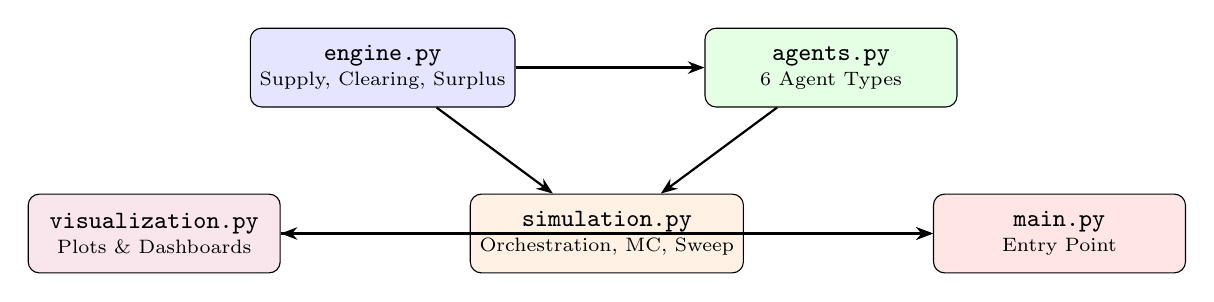
\begin{tikzpicture}[
  module/.style={draw, rounded corners, minimum width=3.2cm, minimum height=1cm, font=\small\ttfamily, align=center},
  arr/.style={-{Stealth[length=6pt]}, thick},
  node distance=1.6cm and 2.4cm,
]
  \node[module, fill=blue!10] (engine) {engine.py\\[-2pt]\scriptsize\rmfamily Supply, Clearing, Surplus};
  \node[module, fill=green!10, right=of engine] (agents) {agents.py\\[-2pt]\scriptsize\rmfamily 6 Agent Types};
  \node[module, fill=orange!10, below=of $(engine)!0.5!(agents)$] (sim) {simulation.py\\[-2pt]\scriptsize\rmfamily Orchestration, MC, Sweep};
  \node[module, fill=purple!10, left=of sim] (viz) {visualization.py\\[-2pt]\scriptsize\rmfamily Plots \& Dashboards};
  \node[module, fill=red!10, right=of sim] (main) {main.py\\[-2pt]\scriptsize\rmfamily Entry Point};

  \draw[arr] (engine) -- (sim);
  \draw[arr] (agents) -- (sim);
  \draw[arr] (sim) -- (viz);
  \draw[arr] (sim) -- (main);
  \draw[arr] (viz) -- (main);
  \draw[arr] (engine) -- (agents);
\end{tikzpicture}
\caption{Module dependency graph.}
\label{fig:architecture}
\end{figure}

\begin{itemize}[nosep]
  \item \textbf{\texttt{engine.py}} --- CCA mechanism primitives: supply schedule construction, three spreading rules, the bisection-based clearing solver, and surplus decomposition.
  \item \textbf{\texttt{agents.py}} --- The six agent types (Section~\ref{sec:agent-types}), the abstract \texttt{BaseAgent} with the conjugate belief-update protocol, the \texttt{MarketState} observable, and the population factory.
  \item \textbf{\texttt{simulation.py}} --- The information model (public signals, sentiment dynamics), the single-run orchestrator (Algorithm~\ref{alg:single-run}), the Monte Carlo runner, and the parameter-sweep infrastructure.
  \item \textbf{\texttt{visualization.py}} --- All plotting routines: the 7-panel single-run dashboard, 4-panel parameter-sweep charts, and 3-panel scenario comparison.
  \item \textbf{\texttt{main.py}} --- Entry point that executes all seven experiments and writes outputs (PNG figures and CSV data files).
\end{itemize}


% ══════════════════════════════════════════════════════════
\section{Mapping to Theory}
\label{sec:mapping}

Table~\ref{tab:mapping} summarises how each theoretical primitive maps to the simulation.

\begin{table}[h]
\centering
\caption{Correspondence between theoretical model and simulation components.}
\label{tab:mapping}
\begin{tabular}{@{}p{4.5cm}p{4.5cm}p{5cm}@{}}
\toprule
\textbf{Theory} & \textbf{Simulation} & \textbf{Reference} \\
\midrule
Discrete time $k \in \{1,\dots,T\}$              & Period loop in Algorithm~\ref{alg:single-run}            & Section~\ref{sec:single-run} \\
Supply increment $q_k$                            & \texttt{build\_supply\_schedule}                          & Section~\ref{sec:supply} \\
Spreading rule $b_k(\tau)$                        & \texttt{proportional\_spreading}                          & Section~\ref{sec:spreading}, Eq.~\eqref{eq:proportional-spread} \\
Clearing price $P_k$ s.t.\ $D(P_k) = q_k$        & \texttt{find\_clearing\_price} (bisection)                & Section~\ref{sec:clearing} \\
Surplus $\pi_k^{(i)}$                             & \texttt{compute\_surplus}                                 & Section~\ref{sec:surplus}, Eq.~\eqref{eq:surplus-period} \\
Prop.~1 (front-loaded surplus $\Rightarrow$ early entry)  & EarlyBeliever behaviour                          & Section~\ref{sec:early-believer} \\
Prop.~2 (option value of waiting)                 & InformedTrader, OptionValueOptimizer             & Sections~\ref{sec:informed-trader},~\ref{sec:option-value} \\
Assumption~1 (price-taking)                       & All agents except WhaleAgent                              & Section~\ref{sec:whale} \\
Assumption~3 (information arrival)                & Private signals, public signal leakage                    & Sections~\ref{sec:informed-trader},~\ref{sec:public-signal} \\
Filtration $\cF_k$                                & \texttt{MarketState} + belief updates                     & Sections~\ref{sec:market-state},~\ref{sec:belief-update} \\
Conditional surplus $g_k(\tau,m)$                 & Emergent from clearing + belief dynamics                   & Sections~\ref{sec:clearing},~\ref{sec:surplus} \\
\bottomrule
\end{tabular}
\end{table}


% ══════════════════════════════════════════════════════════
\section{Implementation Notes}
\label{sec:notes}

\paragraph{Numerical precision.}  The clearing-price bisection converges to $10^{-8}$ relative tolerance in at most 200 iterations.  The demand function~\eqref{eq:demand} is piecewise continuous with discontinuities at each agent's cap; bisection handles this correctly without special treatment.

\paragraph{RNG discipline.}  All randomness flows through \texttt{numpy.random.Generator} objects instantiated with explicit seeds.  Each Monte Carlo run receives seed $\texttt{base\_seed} + \texttt{run\_id}$, and each agent receives its own child generator to avoid cross-contamination.

\paragraph{Computational cost.}  Each single run is $O(T \times N)$, where $N$ is the total number of bids.  The period-by-period loop re-runs the full auction at each step to correctly account for newly entering bids—this is intentional and faithful to the mechanism.  For the default configuration ($T = 24$, $N \approx 70$), a single run completes in under one second; the full experiment suite (including all parameter sweeps with 15~runs each) executes in approximately 90~seconds.

\paragraph{Extensibility.}  The spreading rule is a pluggable function.  New agent types can be added by subclassing \texttt{BaseAgent} and implementing \texttt{decide\_entry} and \texttt{decide\_cap}.  Supply schedules accept arbitrary weight vectors via the \texttt{custom} type.


% ══════════════════════════════════════════════════════════

\end{document}
